\documentclass{beamer}
\usepackage[utf8]{inputenc}
\usepackage[czech]{babel}
\usepackage{hyperref}
\usepackage[noline, czech, longend]{algorithm2e}
\usepackage{setspace}

\usetheme{Warsaw}
\urlstyle{same}

%% OBSAH TITULNI STRANY {
\title{Dijkstrův algoritmus}
\subtitle{nalezení nejkratší cesty v grafu}
\author{Dominik Horký}
\institute{Fakulta Informačních technologií\\Vysoké učení technické v Brně}
\date{2020}
%% }

\begin{document}
%% 0 -> TITULNI STRANKA 
\frame{\titlepage}

%% 1 -> DEFINICE
\begin{frame}{Definice}
\begin{itemize}
    \item \onslide<1->{Konečný algoritmus sloužící k nalezení nejkratší cesty v grafu}
    \item \onslide<1->{Používá se nad kladně ohodnocenými grafy}
    \begin{itemize}
        \item \onslide<2->{neohodnocené grafy lze snadno převést na ohodnocené}
        \item \onslide<2->{pro záporně ohodnocené se používá např. Bellmalův-Fordův algoritmus}
    \end{itemize}
    \item \onslide<3->{Pojmenován podle svého autora Edsgera Dijkstry}
\end{itemize}
\end{frame}

%% 2 -> POSTUP, JAK FUNGUJE, POPIS
\begin{frame}{Popis algoritmu}
\begin{itemize}
    \item \onslide<1->{Všechny vrcholy grafu $G$ (tzv. $d[v]$) z množiny všech vrcholů $V$ nastavíme na $\infty$}
    \item \onslide<2->{Počáteční vrchol ($d[s]$) nastavíme na hodnotu 0}
    \item \onslide<3->{V průběhu algoritmu si zaznamenáváme, které vrcholy jsme už navštívili (množina $Z$) a které nikoliv (množina $N$)}
    \item \onslide<4->{Algoritmus cyklí tak dlouho, dokud $N$ není prázdnou množinou}
    \item \onslide<5->{V každém průchodu cyklu se přidá jeden vrchol z $N$ do $Z$ takový, který má nejmenší hodnotu $d[v]$ ze všech vrcholů v $N$}
    \item \onslide<6->{Po skončení algoritmu je délka nejkratší cesty uložena v $d[v]$}
\end{itemize}
\end{frame}

%% 3.1 -> PSEUDOKOD - TEXT
\begin{frame}{Pseudokód}
Celý algoritmus lze však (mnohem lépe) pochopit z pseudokódu.
\end{frame}

%% 3.2 -> PSEUDOKOD - KOD
\begin{frame}{Pseudokód (jazyk Pascal)}
\IncMargin{0.5em}
\begin{algorithm}[H]
\setstretch{0.86}
\SetNlSty{}{}{:}
\SetAlgoNlRelativeSize{0}

\Indp \Indpp
\SetInd{1em}{1em}
\BlankLine
\Indm \Indmm
$function\ Dijkstra (E, V, s)$\\
\Indp \Indpp
\For{\textbf{each} vertex v \textbf{in} V}{
    $d[v] := \infty$\\
    $p[v] := undefined$\\
}
$d[s] := 0$\\
$N := V$\\
\While{N \textbf{is not} empty}{
    $u := extract\_min(N)$\\
    \For{\textbf{each} neighbor v \textbf{of} u}{
    $alt = d[u] + l(u, v)$\\
    \If{$alt < d[v]$}{
        $d[v] := alt$\\
        $p[v] := u$\\
        }
    }
}
\end{algorithm}

\end{frame}

%% 4 -> SLOZITOST
\begin{frame}{Složitost}
\begin{itemize}
    \item Samotný algoritmus není pro implementaci příliš složitý
    \item Lze jej naimplementovat s asymptotickou časovou složitostí:
    $$O(E + V \log V)$$\\[1em]
    \item $|V|$ je počet uzlů, $|E|$ je počet hran
\end{itemize}
\end{frame}

%% 5 -> SLOZITOST - OPTIMALIZACE
\begin{frame}{Složitost - řídké grafy}
\begin{itemize}
    \item \onslide<1->{Algoritmus lze optimalizovat pro tzv. řídké grafy (ty, které mají $|E| < |V|^2$)}
    \onslide<2->{
    \begin{itemize}
        \item graf se uloží podle seznamu sousedů
        \item funkci $extract\_min$ implementujeme pomocí Fibonacciho nebo binární haldy
    \end{itemize}
    }
    \onslide<3->{\item Po těchto optimalizacích algoritmus běží v čase:
    $$O( (|E| + |V|) \log |V| )$$
    }
\end{itemize}
\end{frame}

%% 6.1 -> PRIKLAD POUZITI - P1
\begin{frame}{Příklad použití algoritmu (1/3)}
    \begin{center}
    \scalebox{0.4}{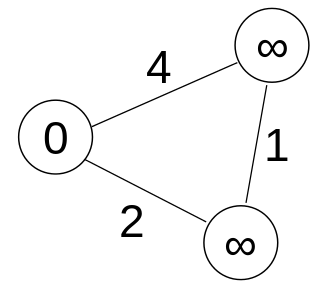
\includegraphics{data/graph_1.png}}\\[1em]
    Počáteční vrchol nastavíme na hodnotu 0, ostatní na $\infty$
    \end{center}
\end{frame}

%% 6.2 -> PRIKLAD POUZITI - P2
\begin{frame}{Příklad použití algoritmu (2/3)}
    \begin{center}
    \scalebox{0.4}{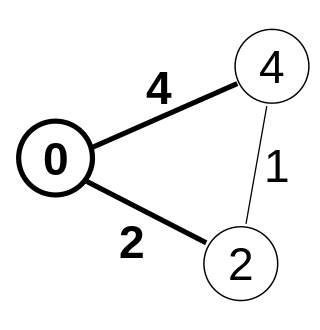
\includegraphics{data/graph_2.png}}\\[1em]
    Nastavíme hodnoty vrcholů dle ohodnocení hran vedoucích k nim
    \end{center}
\end{frame}

%% 6.3 -> PRIKLAD POUZITI - P3
\begin{frame}{Příklad použití algoritmu (3/3)}
    \begin{center}
    \scalebox{0.4}{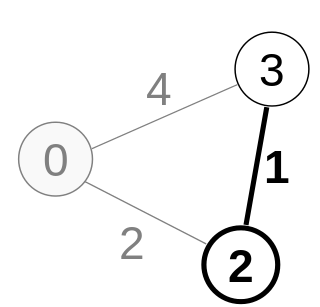
\includegraphics{data/graph_3.png}}\\[1em]
    Nejkratší cesta tohoto malého váženého grafu má hodnotu 3
    \end{center}
\end{frame}

%% 7 -> POUZITI V PRAXI
\begin{frame}{Praxe, využití, závěr}
\begin{itemize}
    \item \onslide<1->{Vhodné je implementovat algoritmus spolu s prioritní frontou}
    \item \onslide<2->{Dijkstrův algoritmus lze použít při hledání nejkratší cesty na mapách}
    \item \onslide<2->{Algoritmus je nicméně pro reálné využití v mapách (jako např. Google Maps) příliš pomalý}
    \item \onslide<3->{Nejčastěji je tak využitý zejména v hledání nejkratších cest grafů}
\end{itemize}
\end{frame}

%% POUZITE ZDROJE
\begin{frame}{Použité zdroje}
\begin{itemize}
\setlength{\parskip}{0.3em}
    \item Algoritmus, pseudokód \\[0.2em]
    \small{\url{https://cs.wikipedia.org/wiki/Dijkstr\%C5\%AFv\_algoritmus}}
    \item Dodatečné informace \\[0.2em]
    \small{\url{http://voho.eu/wiki/algoritmus-dijkstra/}}
    \item Obrázky (graf použitý v příkladu) \\[0.2em]
    \small{\url{https://upload.wikimedia.org/wikipedia/commons/thumb/b/be/Dijkstra\%27s\_algorithm.svg/100px-Dijkstra\%27s\_algorithm.svg.png}}
    \item Použití v praxi \\[0.2em]
    \small{\url{https://is.mendelu.cz/eknihovna/opory/zobraz_cast.pl?cast=19938}}
\end{itemize}
\end{frame}

%%%%%%%%%%% TODO SLIDE END
\end{document}
